\section{Übersicht}

\begin{frame}
  {Übersicht}
  \onslide<+->
  \begin{itemize}[<+->]
    \item \citet{Schaefer2018b}
  \end{itemize}
\end{frame}

\section[Wortzeichen]{Vergessen: Wortzeichen}

\begin{frame}
  {--}
  \onslide<+->
  \onslide<+->
  \begin{exe}
    \ex
    \begin{xlist}
      \ex[ ]{Wohnungstür}
      \ex[*]{Wohnung\orongsch{s}-Tür}
    \end{xlist}
    \ex
    \begin{xlist}
      \ex[ ]{Ofenkammer}
      \ex[?]{Ofen-Kammer}
    \end{xlist}
    \ex
    \begin{xlist}
      \ex[?]{Hornerschema}
      \ex[ ]{Horner-Schema}
    \end{xlist}
    \ex
    \begin{xlist}
      \ex[?]{Xylitsüßmittel}
      \ex[ ]{Xylit-Süßmittel}
    \end{xlist}
    \ex
    \begin{xlist}
      \ex[*]{Mallocexception}
      \ex[ ]{Malloc-Exception}
    \end{xlist}
  \end{exe}
\end{frame}

\begin{frame}
  {Der Bindestrich}
  \onslide<+->
  \begin{itemize}[<+->]
    \item Kompositum = \alert{ein} syntaktisches\slash prosodisches Wort,\\
      \onslide<+->
      \alert{zwei} phonologische\slash morphologische Wörter
      \Halbzeile
    \item Spatium | Trennung syntaktischer Wörter
      \Zeile
    \item Bindestrich | optionaler morpholgischer Trenner im Kompositum
      \begin{itemize}[<+->]
        \item weitgehend \rot{blockiert bei Fugenelemnt}
        \item prototypisch bei \alert{Eigennamenbeteiligung}
        \item prototypisch bei \alert{Lehnwortbeteiligung}
        \item präferierter bei stark \tuerkis{produktiver Bildung}
        \item präferierter bei \tuerkis{weniger integrierten Gliedern}
      \end{itemize}
  \end{itemize}
\end{frame}

\begin{frame}
  {`}
  \onslide<+->
  \onslide<+->
  \begin{exe}
    \ex 
    \begin{xlist}
      \ex[ ]{Platz \alert{am} Wilden Eber}
      \ex[*]{Platz \rot{a'm} Wilden Eber}
    \end{xlist}
    \ex 
    \begin{xlist}
      \ex[ ]{\alert{Weißte}, was passiert ist?}
      \ex[*]{\rot{Weißt'e}, was passiert ist?}
    \end{xlist}
    \ex 
    \begin{xlist}
      \ex[ ]{Ich \alert{hab} einen Volvo Amazon.}
      \ex[?]{Ich \orongsch{hab'} einen Volvo Amazon.}
    \end{xlist}
    \ex 
    \begin{xlist}
      \ex[ ]{Wie \alert{gehts}?}
      \ex[ ]{Wie \alert{geht's}?}
    \end{xlist}
  \end{exe}
\end{frame}

\begin{frame}
  {Der Apostroph}
  \onslide<+->
  \begin{itemize}[<+->]
    \item \rot{kein Auslassungszeichen}
    \item \rot{kein allgemeines Klitisierungszeichen}
      \Zeile
    \item optionaler \alert{morphologischer Trenner}
      \begin{itemize}[<+->]
        \item bei \alert{Klitika unter bestimmten Bedingungen}
          \Viertelzeile
        \item präferiert bei \alert{produktiver Klitisierung}
        \item nur möglich bei \alert{ausreichend rekonstruierbaren Klitikon}
        \item unmöglich bei \rot{lexikalisierten Klitisierungen}
          \Zeile
        \item siehe auch \citet{SchaeferSayatz2014} zu \textit{nen} usw.
      \end{itemize}
  \end{itemize}
\end{frame}


\section[Satzschluss]{Sogenannte Satzschlusszeichen}

\begin{frame}
  {.}
  \onslide<+->
  \onslide<+->
  \begin{exe}
    \ex
    \begin{xlist}
      \ex[ ]{Der Rottweiler bellt.}
      \ex[*]{Der Rottweiler bellt}
    \end{xlist}
    \ex
    \begin{xlist}
      \ex[*]{Halt.}
      \ex[*]{Halt}
    \end{xlist}
    \ex
    \begin{xlist}
      \ex[?]{Er nahm den Mantel. Weil kalt.}
      \ex[?]{Er nahm den Mantel, weil kalt.}
    \end{xlist}
  \end{exe}
\end{frame}

\begin{frame}
  {Der Satzschlusspunkt}
  \onslide<+->
  \begin{itemize}[<+->]
    \item unabhängige Sätze
      \begin{itemize}[<+->]
        \item finites Verb im Verbkomplex
        \item alle Dependenten (Ergänzungen und Angaben)
        \item maximale Extraktionsdomäne (auch Fernabhängigkeiten)
        \item Marker logischer Relationen nur Adverben\slash Partikeln
        \item sprechaktfähig, illokutionäre Kraft
      \end{itemize}
      \Zeile
    \item Punkt als \alert{echter Satztrenner ohne besondere Modusmarkierung}
    \item eventuelle atypische Funktion bei Nicht-Sätzen (s.\,u.)
  \end{itemize}
\end{frame}

\begin{frame}
  {! und ?}
  \onslide<+->
  \onslide<+->
  \begin{exe}
    \ex 
    \begin{xlist}
      \ex[ ]{Haben wir noch Zigarren?}
      \ex[*]{Haben wir noch Zigarren.}
      \ex[ ]{Wie bitte?}
      \ex[*]{Wie bitte.}
      \ex[ ]{Wer?}
      \ex[*]{Wer.}
    \end{xlist}
    \ex 
    \begin{xlist}
      \ex[ ]{Joanna Newsom hat ein neues Album!}
      \ex[ ]{Joanna Newsom hat ein neues Album.}
      \ex[ ]{Hurra!}
      \ex[?]{Hurra.}
      \ex[ ]{Gib das her!}
      \ex[ ]{Gib das her.}
    \end{xlist}
  \end{exe}
\end{frame}

\begin{frame}
  {Frage- und Ausrufungszeichen}
  \onslide<+->
  \begin{itemize}[<+->]
    \item beiden gemein
      \begin{itemize}[<+->]
        \item \alert{können} Sätze abschließen
        \item \alert{müssen aber nicht} (auch nicht-satzförmnige Sprechchakte)
      \end{itemize}
      \Zeile
    \item Fragezeichen
      \begin{itemize}[<+->]
        \item markiert interrogativen Sprechaktmodus
        \item dabei \alert{obligatorisch}
      \end{itemize}
      \Zeile
    \item Ausrufungszeichen
      \begin{itemize}[<+->]
        \item markiert exklamativen Sprechaktmodus
        \item dabei stärker \alert{optional} | durch Punkt ersetzbar
        \item aber Punkt ggf.\ hoch atypisch bei Nicht-Sätzen
      \end{itemize}
  \end{itemize}
\end{frame}

\section{Rest}

\begin{frame}
  {;}
  \onslide<+->
  \begin{itemize}[<+->]
    \item laut Rechtschreibregeln
      \Halbzeile
      \begin{itemize}[<+->]
        \item Listen von Wortgruppen\\
          \grau{Pfeffer und Salz; Rosmarin und Thymian; Basilikum und Oregano}
          \Halbzeile
        \item nicht so ganz unabhängige Sätze(?)\\
          \grau{}
          \Halbzeile
        \item \rot{immer optional}
        \item deswegen auch weitgehend dispräferiert
      \end{itemize}
  \end{itemize}
\end{frame}

\begin{frame}
  {Idioten in der SZ (I)}
  \footnotesize
  SZ Magazin 10.07.2008, \textit{Ein gutes Zeichen} von Johannes Waechter\\
  \Zeile
  Auf Thomas Mann ist wenigstens Verlass. Schon im zweiten Satz des Zauberbergs hat der Altmeister der Interpunktion das erste Semikolon platziert; das nächste folgt nur einen Satz später. So geht es weiter, tausend Seiten lang, bis Hans Castorp im Pulverdampf des Ersten Weltkriegs verschwindet, dabei selbstredend von zahlreichen Strichpunkten flankiert.\\
  \ldots\\
  Die Betonung liegt auf »kann«. Anders gesagt: Keine Satzkonstruktion ist denkbar, in der ein Semikolon Pflicht wäre; stets bleibt die Entscheidung dem Sprachgefühl und der Initiative des Schreibenden überlassen – der dann in der Regel das Komma vorzieht.\\
  \ldots\\
  In Frankreich, wo man seit Proust ein nahezu libidinöses Verhältnis zum \textit{point-virgule} pflegt, werden indes noch andere Gründe diskutiert. Französische Intellektuelle entdecken die Totengräber des Semikolons dort, wo der ganze restliche Ungeist herkommt: in den USA. Die amerikanische Sprache mit ihren kurzen Hauptsätzen mache dem Semikolon den Garaus; die Popkultur mit ihrer Ästhetik der Oberfläche tue ein Übriges, um komplexe Analysen und längliche Gedankengänge, die sich nur mithilfe von Strichpunkten aufschreiben ließen, gar nicht erst aufkommen zu lassen.\\
  \ldots\\
\end{frame}

\begin{frame}
  {Idioten in der SZ (II)}
  \footnotesize
  SZ Magazin 10.07.2008, \textit{Ein gutes Zeichen} von Johannes Waechter\\
  \Zeile
  Zum Glück hält Michel Houellebecq als einer der letzten Virtuosen des Semikolons die Fahne hoch: »Sie trug ein kurzes, hautenges, makellos weißes Kleid«, schreibt er in Ausweitung der Kampfzone, »das der Schweiß an ihren Körper geklebt hatte; darunter trug sie, wie man sehen konnte, nichts; ihr kleiner runder Hintern war perfekt geformt; deutlich zu erkennen die braunen Höfe ihrer Brüste.«\\
  \ldots\\
  Alles in allem erscheint der Niedergang des Semikolons somit als Symptom der Angepasstheit unserer Epoche. Von der Freizeitkultur des Denkens entwöhnt, können wir zwar noch wählen, etwa wenn wir im Elektronikmarkt einen von 35 Flachbildschirmen auswählen; aber wir haben weder den Mut noch den Instinkt, uns zu entscheiden; und sei es nur für ein Semikolon statt eines Kommas.\\
  \Zeile
  \onslide<+->
  \onslide<+->
  Dazu ich so: \alert{Thoman Mann; Michel Houellebecq; Johannes Waechter\ldots\ Kotz!}
\end{frame}


\begin{frame}
  {Parenthesemarker}
  \begin{itemize}[<+->]
    \item Konkurrenz von
      \begin{itemize}[<+->]
        \item Klammer\\
          \textit{\alert{der (wenig brauchbare) Artikel}}
        \item Gedankenstrich\\
          \textit{\alert{der -- wenig brauchbare -- Artikel}}
        \item paarigem Komma\\
          \textit{\alert{der, wenig brauchbare, Artikel}}
      \end{itemize}
      \Zeile
    \item Fuhrhop: ``pränominale Herausstellung ist Domäne des Gedankenstrichs''
      \begin{itemize}[<+->]
        \item Pärskription oder Deskription?
        \item wissenschaftliche Graphematik?
      \end{itemize}
  \end{itemize}
\end{frame}

\section[Herausstellung]{Markierung pränominaler Herausstellung | Sayatz \& Schäfer i.V.}

\begin{frame}
  {Konzept der \orongsch{Gebrauchsbasierten Graphematik}}
  \begin{itemize}[<+->]
    \item Regeln (Orthographie)
      \begin{itemize}[<+->]
        \item regelhafte Grammatik
        \item regelhafte Abbildung auf Schreibung
        \item nur Schriftsprache
        \item und bei \rot{Regelungslücken?}
      \end{itemize}
      \Halbzeile
    \item Gebrauchsbasierte Grammatik
      \begin{itemize}[<+->]
        \item Spracherwerb = kognititve Fähigkeiten + Input
        \item Ableiten von \alert{generalisierbaren Regularitäten} aus Input
      \end{itemize}
      \Halbzeile
    \item Gebrauchsbasierte Graphematik
      \begin{itemize}[<+->]
        \item normferne (teilweise auch normnahe) Grammatik
        \item \rot{keine Regeln verfügbar}
        \item Verschriftung = \alert{direkte Folge der gelernten Generalisierungen}
        \item Einblick in Regularitäten der \alert{kognitiven Grammatik}
      \end{itemize}
      \Halbzeile
    \item \grau{auch: \citet{SchaeferSayatzBuch}}
  \end{itemize}
\end{frame}

\begin{frame}
  {Diktatexperiment | Experimentdesign}
  \citet{SayatzSchaeferHerausstellung}\\
  \Zeile
  \centering 
  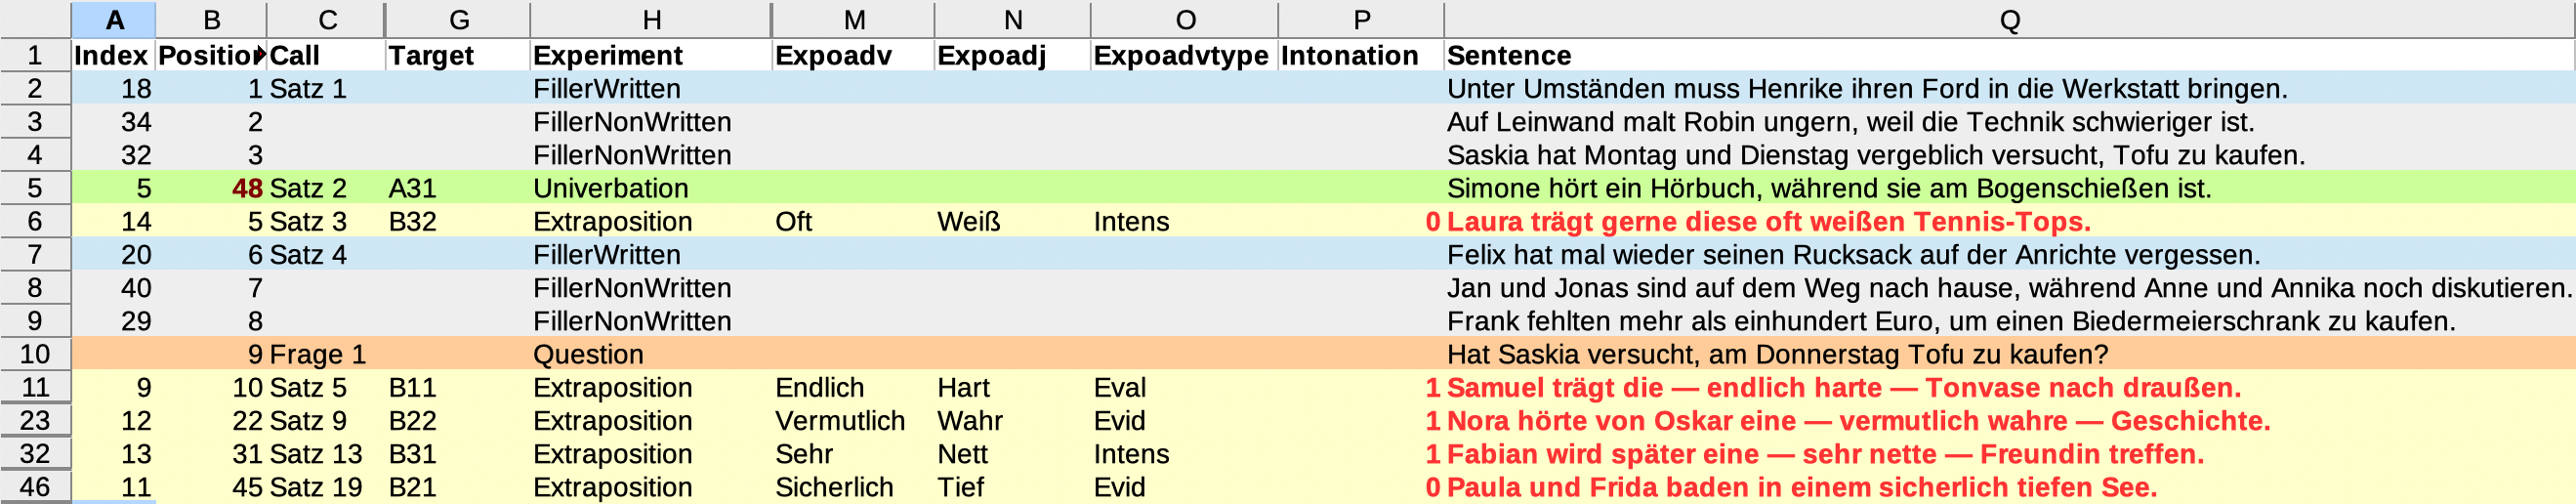
\includegraphics[width=1\textwidth]{\GRAPHPATH/Herausstellung/experiment}
\end{frame}

\begin{frame}
  {Diktatexperiment | Ergebnisse (1)}
  \centering 
  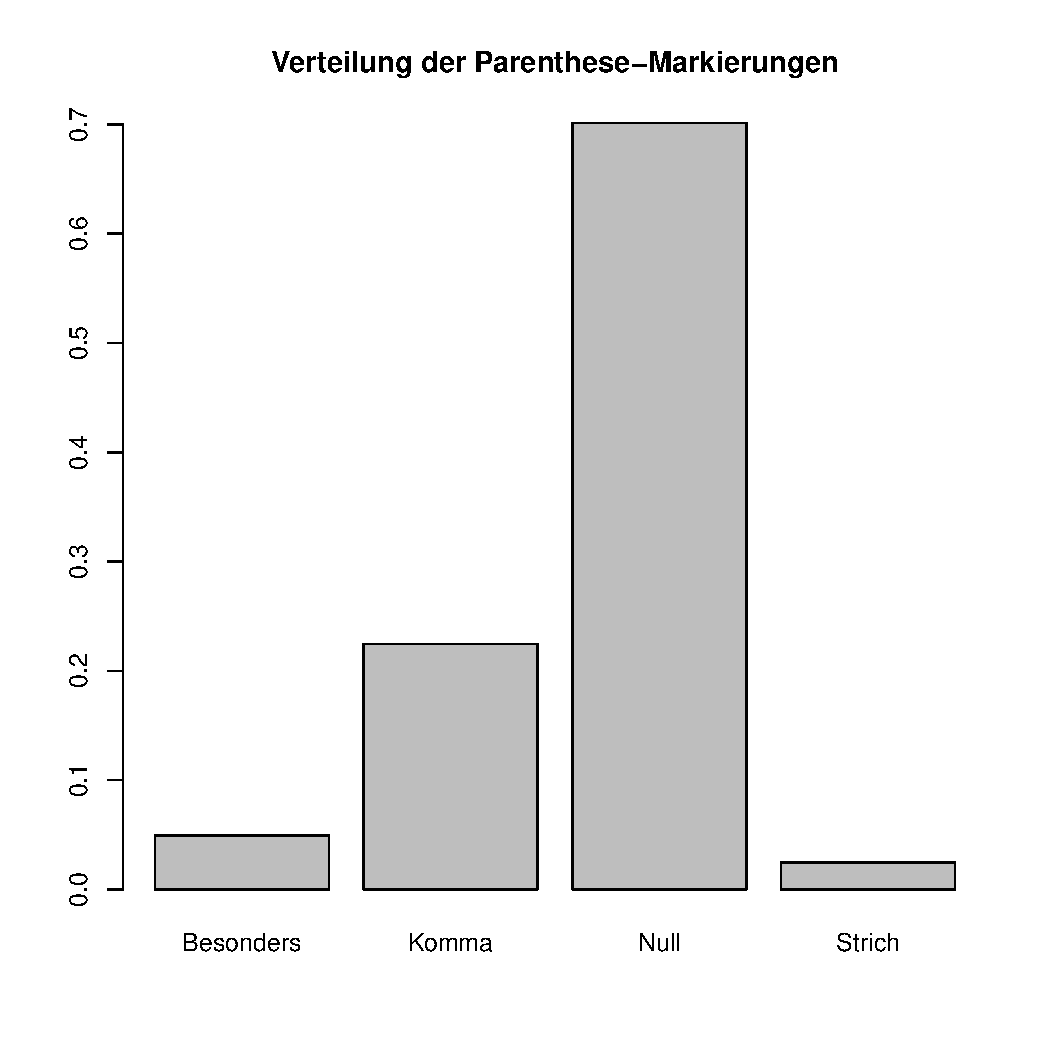
\includegraphics[width=0.5\textwidth]{\GRAPHPATH/Herausstellung/markierungen}
\end{frame}

\begin{frame}
  {Diktatexperiment | Ergebnisse (2)}
  \centering 
  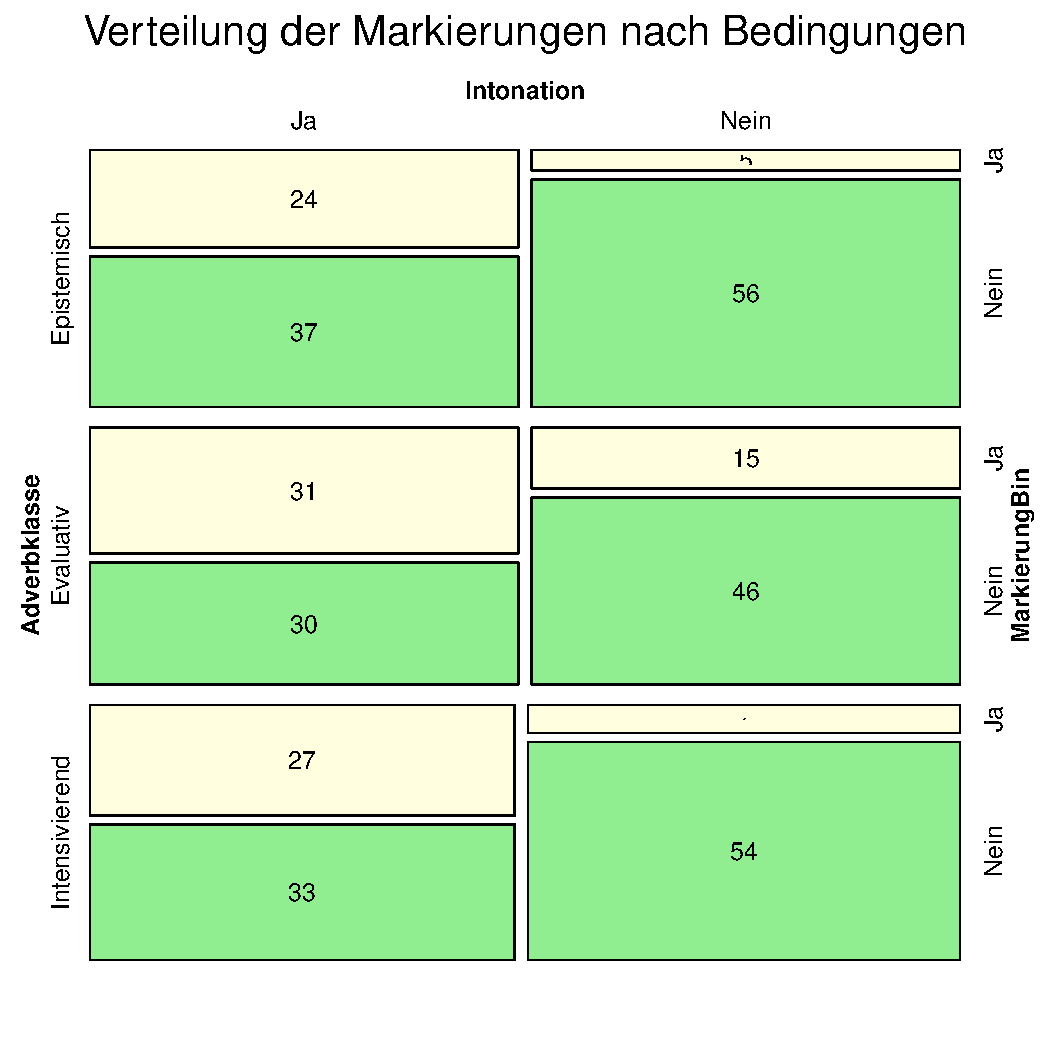
\includegraphics[width=0.5\textwidth]{\GRAPHPATH/Herausstellung/responses}
\end{frame}


\begin{frame}
  {Ergebnisse}
  \begin{itemize}[<+->]
    \item Markierung mit Komma und Gedankenstrich
    \item Komma im Experiment präferiert\\
      \grau{widerspricht Korpusstudie: über 75\% Gedankenstrich}
      \Halbzeile
    \item Intonation vertärkt Tendenz zu Markierung
    \item die Adverbklasse wirkt auch als Auslöser
      \Halbzeile
    \item Funktion?
  \end{itemize}
\end{frame}

\section[Unabhängigkeit]{Unabhängigkeit von Sätzen | \citet{SchaeferSayatz2016}}


\begin{frame}
  {\textit{obwohl} und \textit{weil} mit V2}
  \citet{SchaeferSayatz2016}\\
  \Zeile
  \centering 
  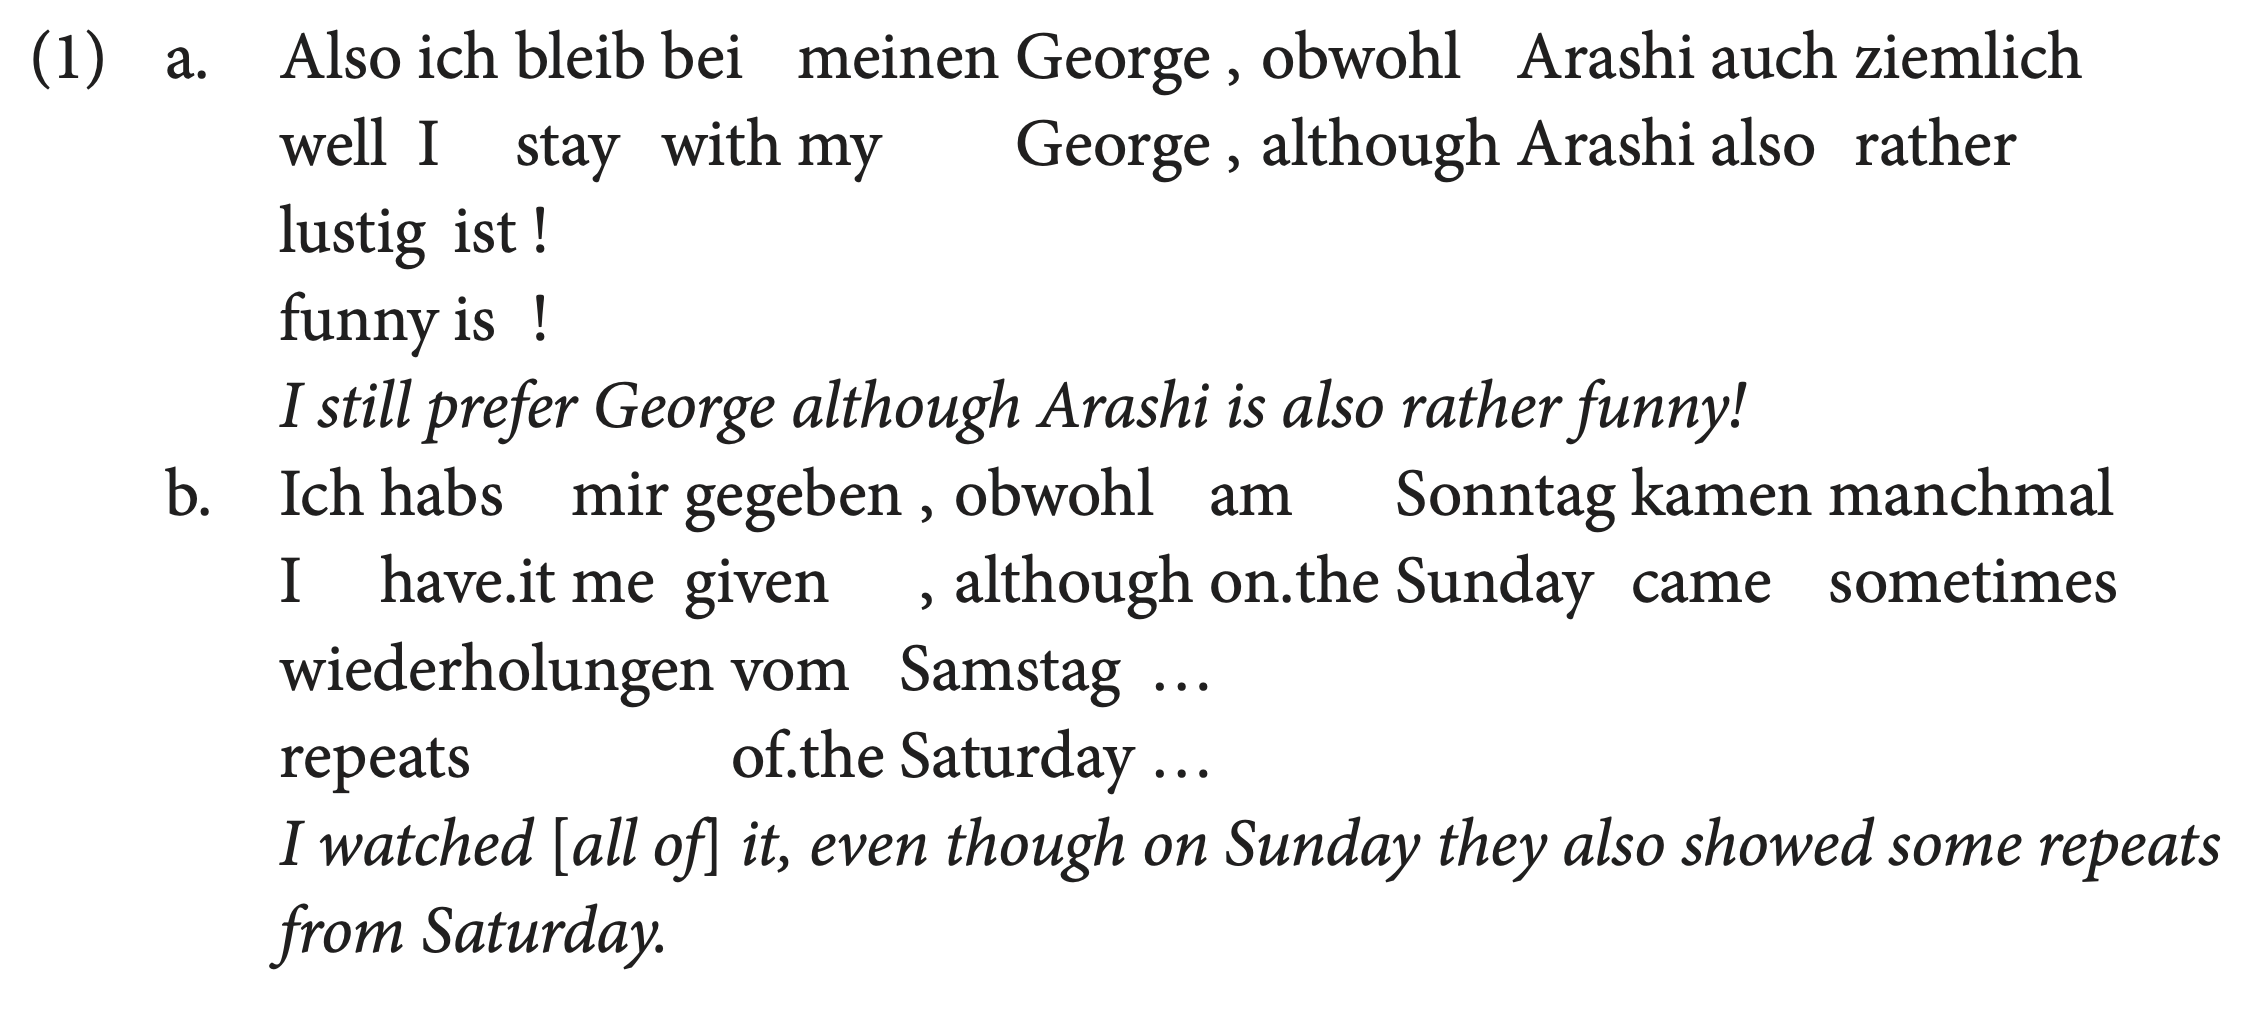
\includegraphics[width=0.7\textwidth]{\GRAPHPATH/obweil/01-obwohl}
\end{frame}

\begin{frame}
  {\textit{obwohl} und \textit{weil} mit V2}
  \centering 
  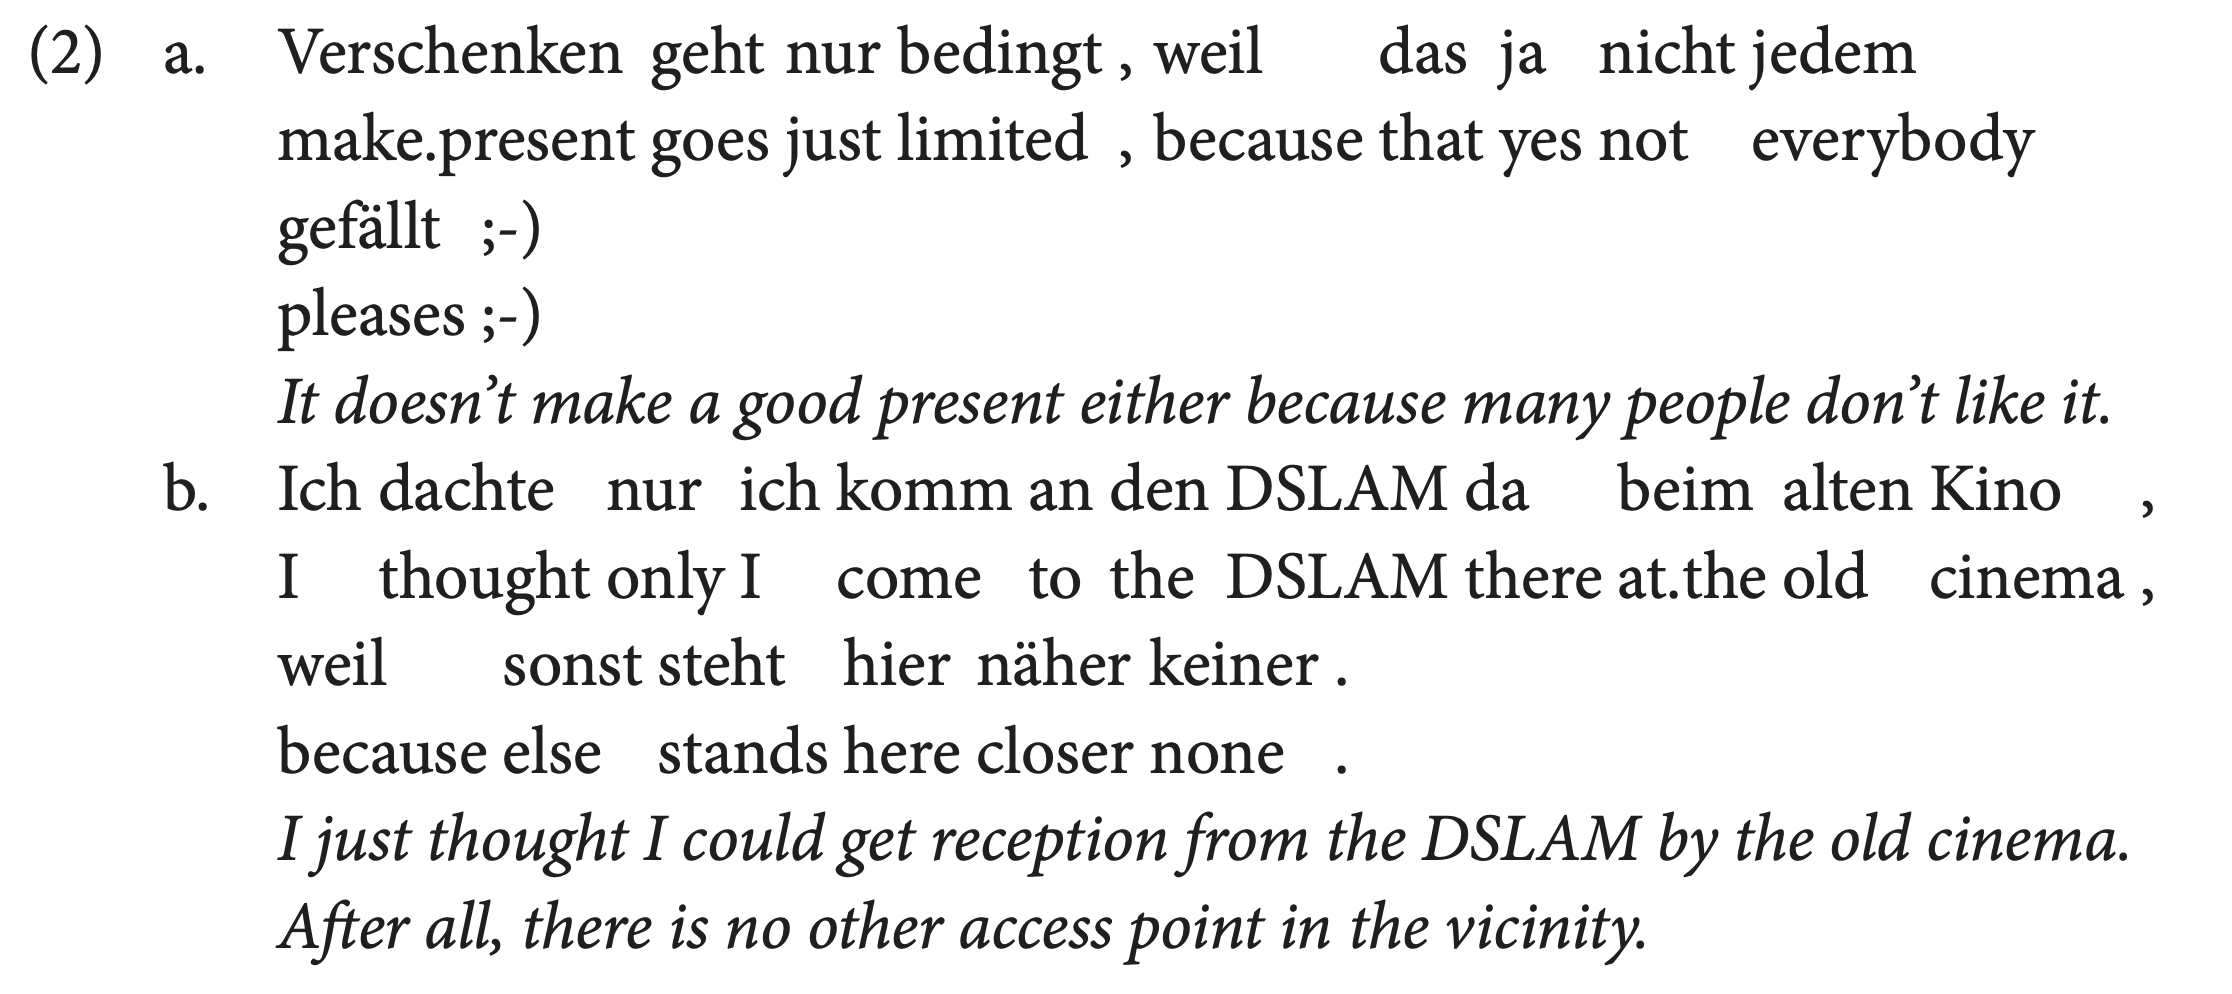
\includegraphics[width=0.7\textwidth]{\GRAPHPATH/obweil/01-weil}
\end{frame}

\begin{frame}
  {Variation der Interpunktion (Beispiele)}
  \centering 
  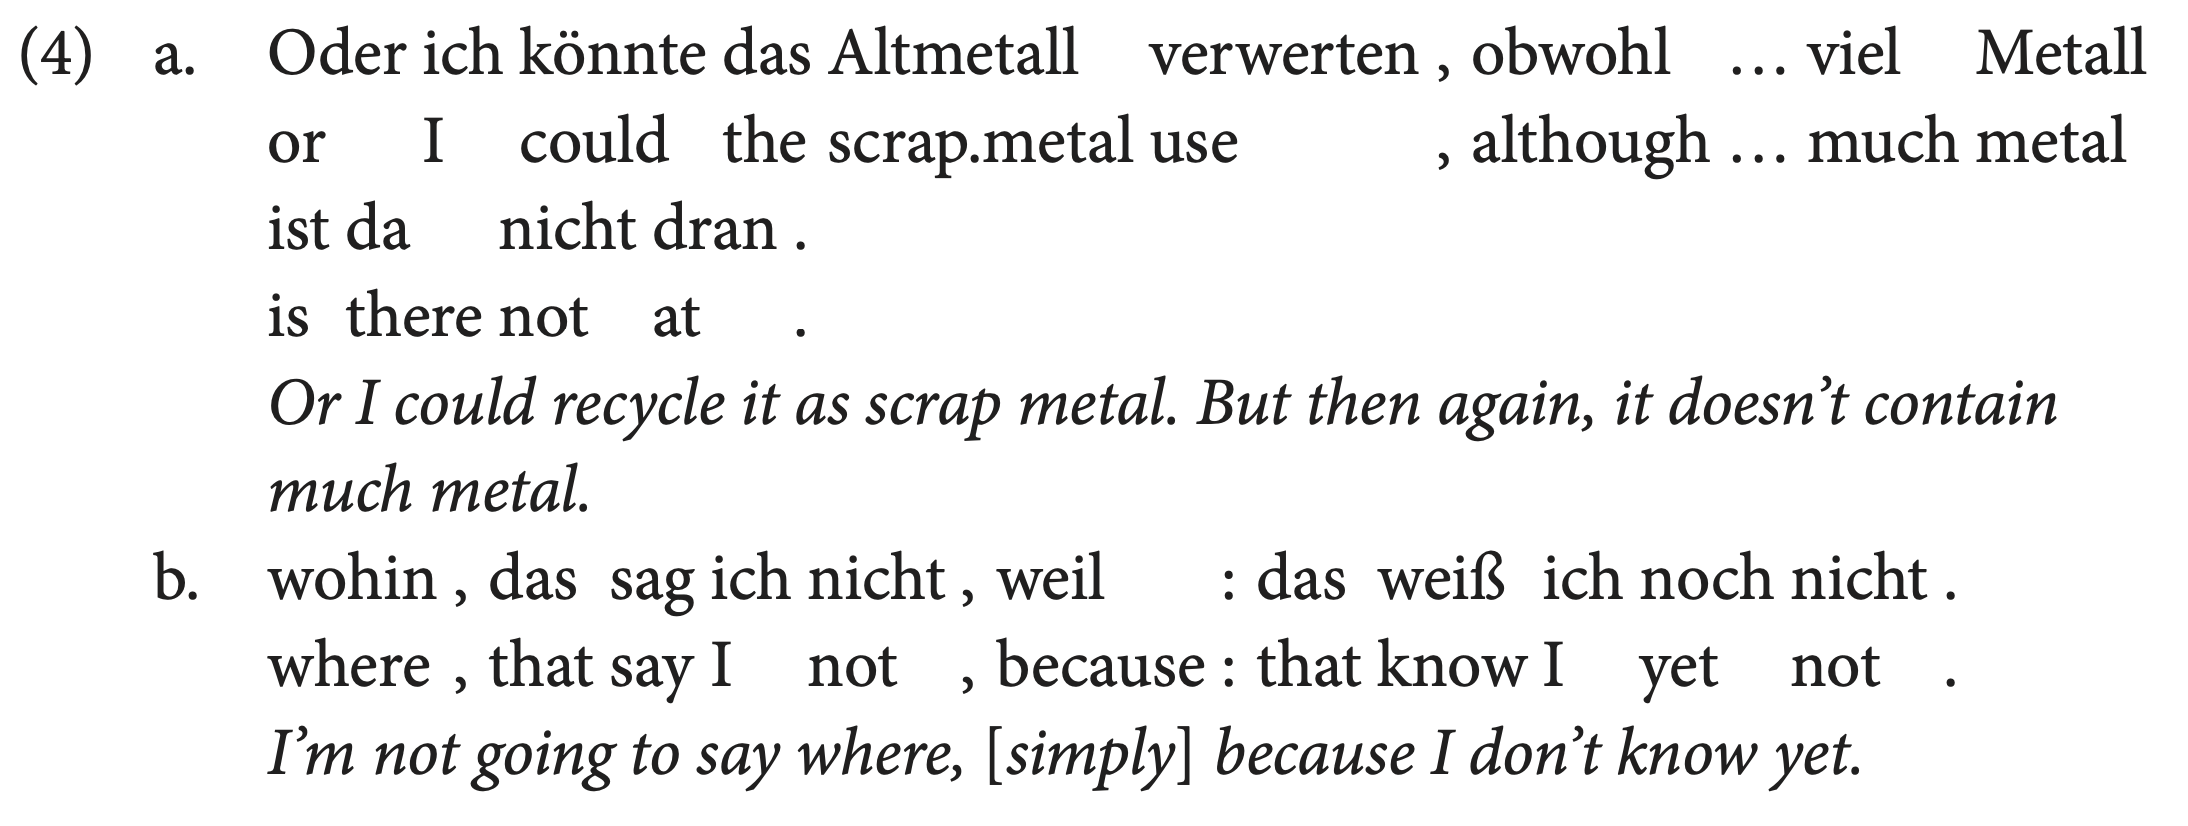
\includegraphics[width=0.7\textwidth]{\GRAPHPATH/obweil/02-interpunktion}
\end{frame}

\begin{frame}
  {Unabhängigkeit von Sätzen}
  \centering 
  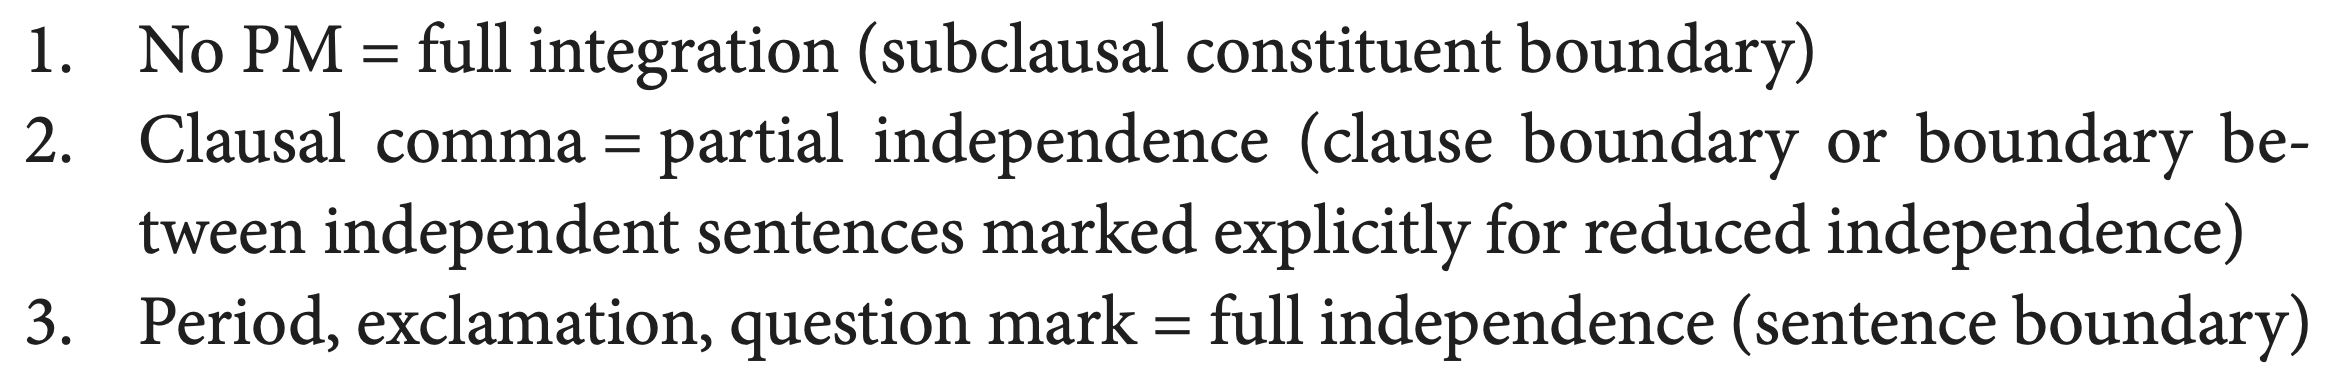
\includegraphics[width=0.7\textwidth]{\GRAPHPATH/obweil/03-independence} 
\end{frame}

\begin{frame}
  {Empirischer Befund I | Satzinitiale Partikeln}
  \centering 
  
\includegraphics[width=0.7\textwidth]{\GRAPHPATH/obweil/04-satzinitial}
\end{frame}

\begin{frame}
  {Empirischer Befund II/1 | Wortverteilung bei Doppelpunkt}
  \centering 
  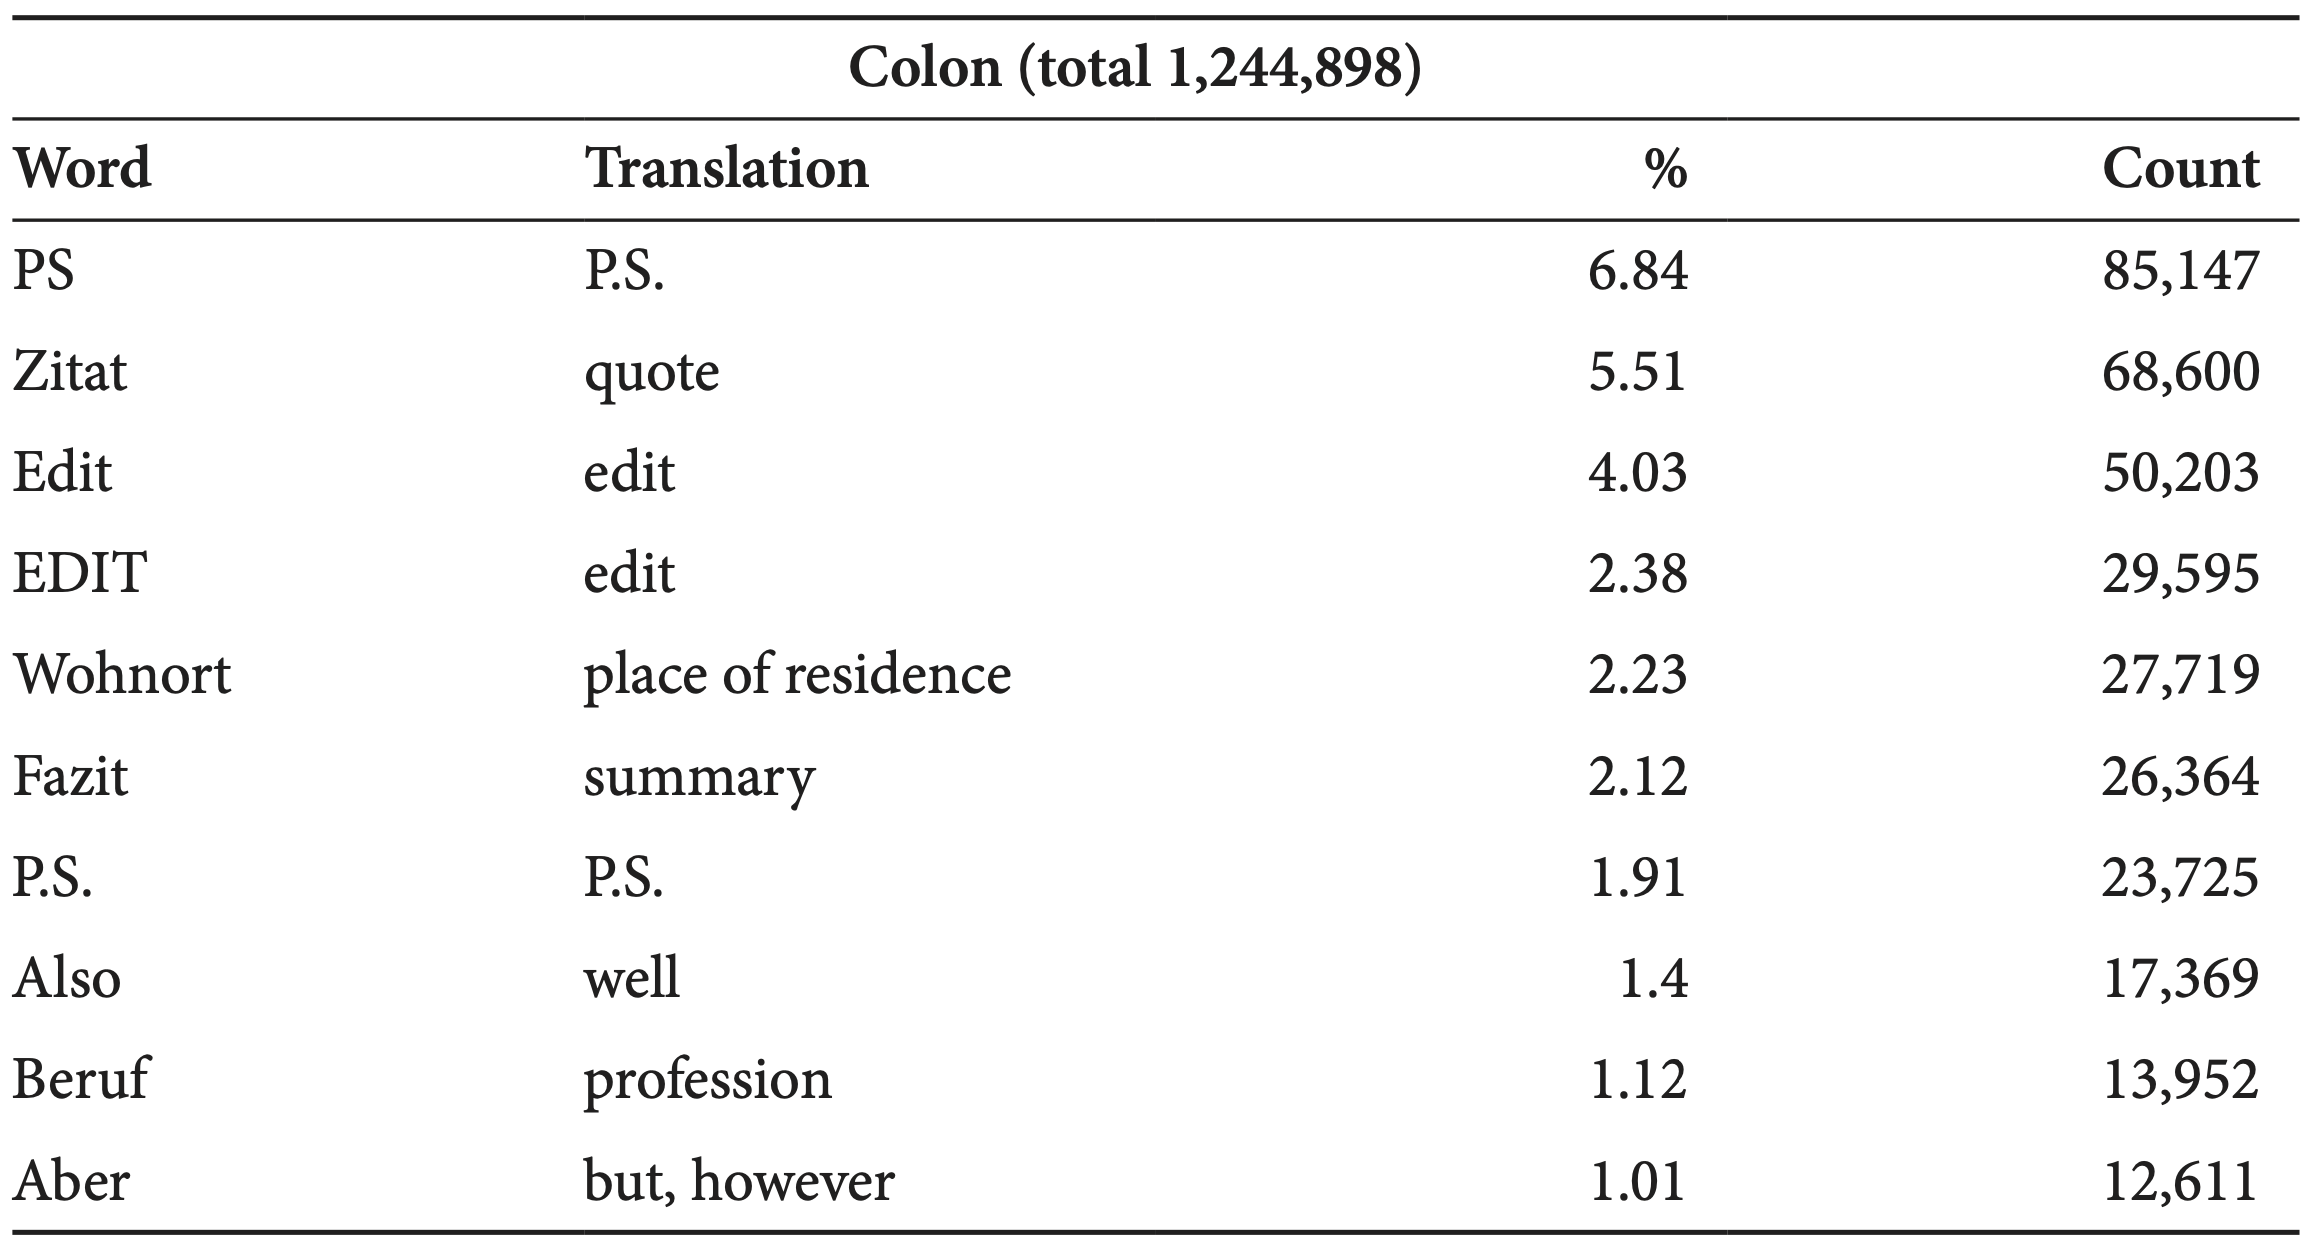
\includegraphics[width=0.7\textwidth]{\GRAPHPATH/obweil/05-colon}
\end{frame}

\begin{frame}
  {Empirischer Befund II/2 | Wortverteilung bei Komma}
  \centering 
  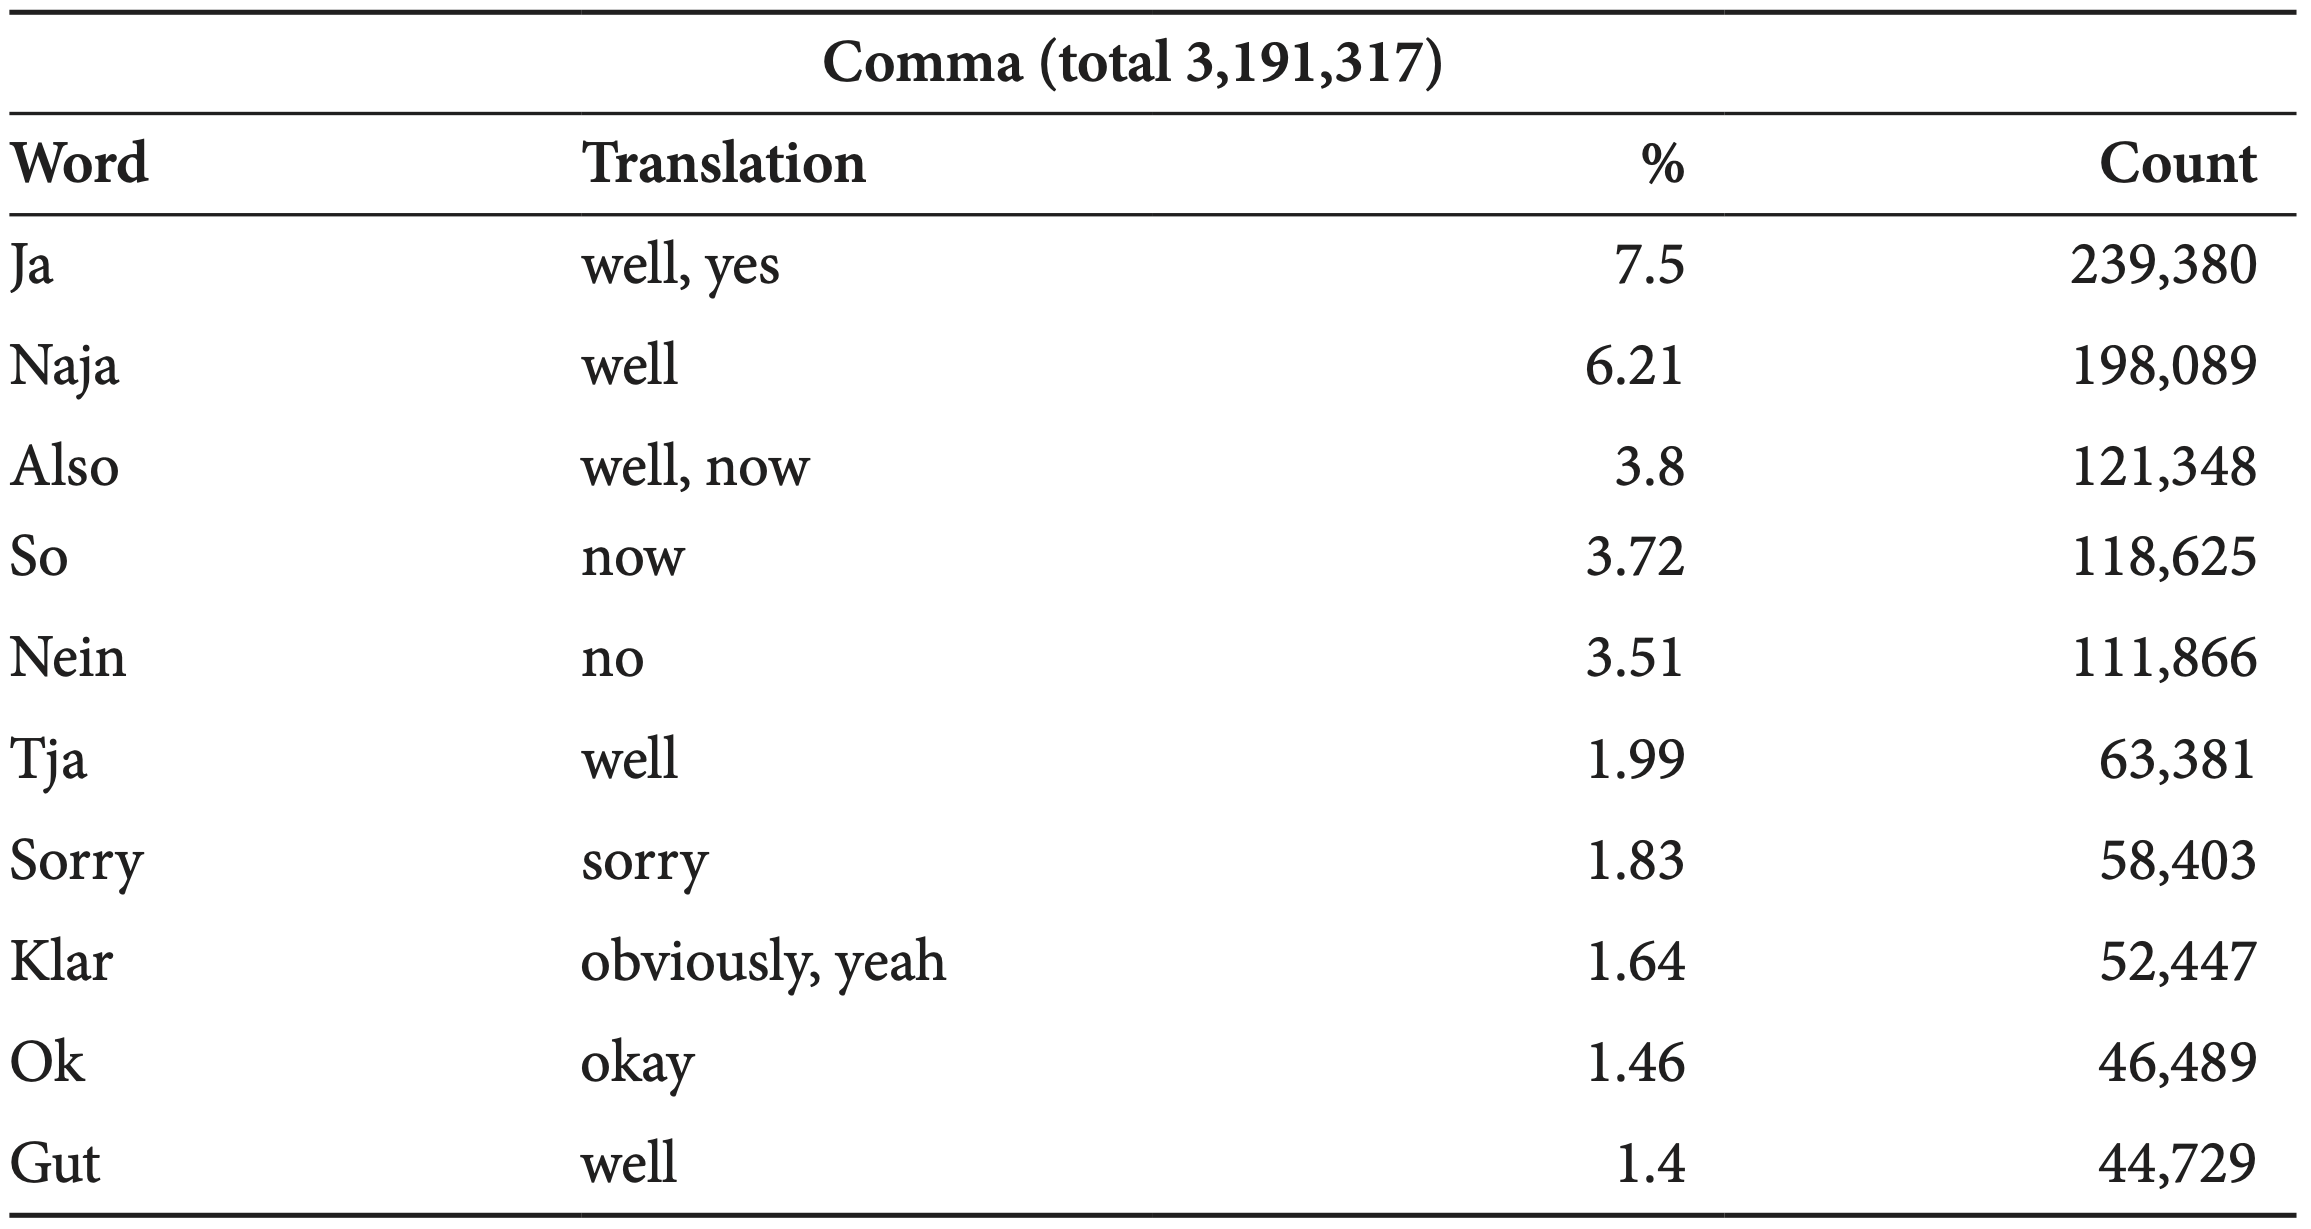
\includegraphics[width=0.7\textwidth]{\GRAPHPATH/obweil/05-comma}
\end{frame}

\begin{frame}
  {Empirischer Befund II/3 | Wortverteilung bei Bindestrich}
  \centering 
  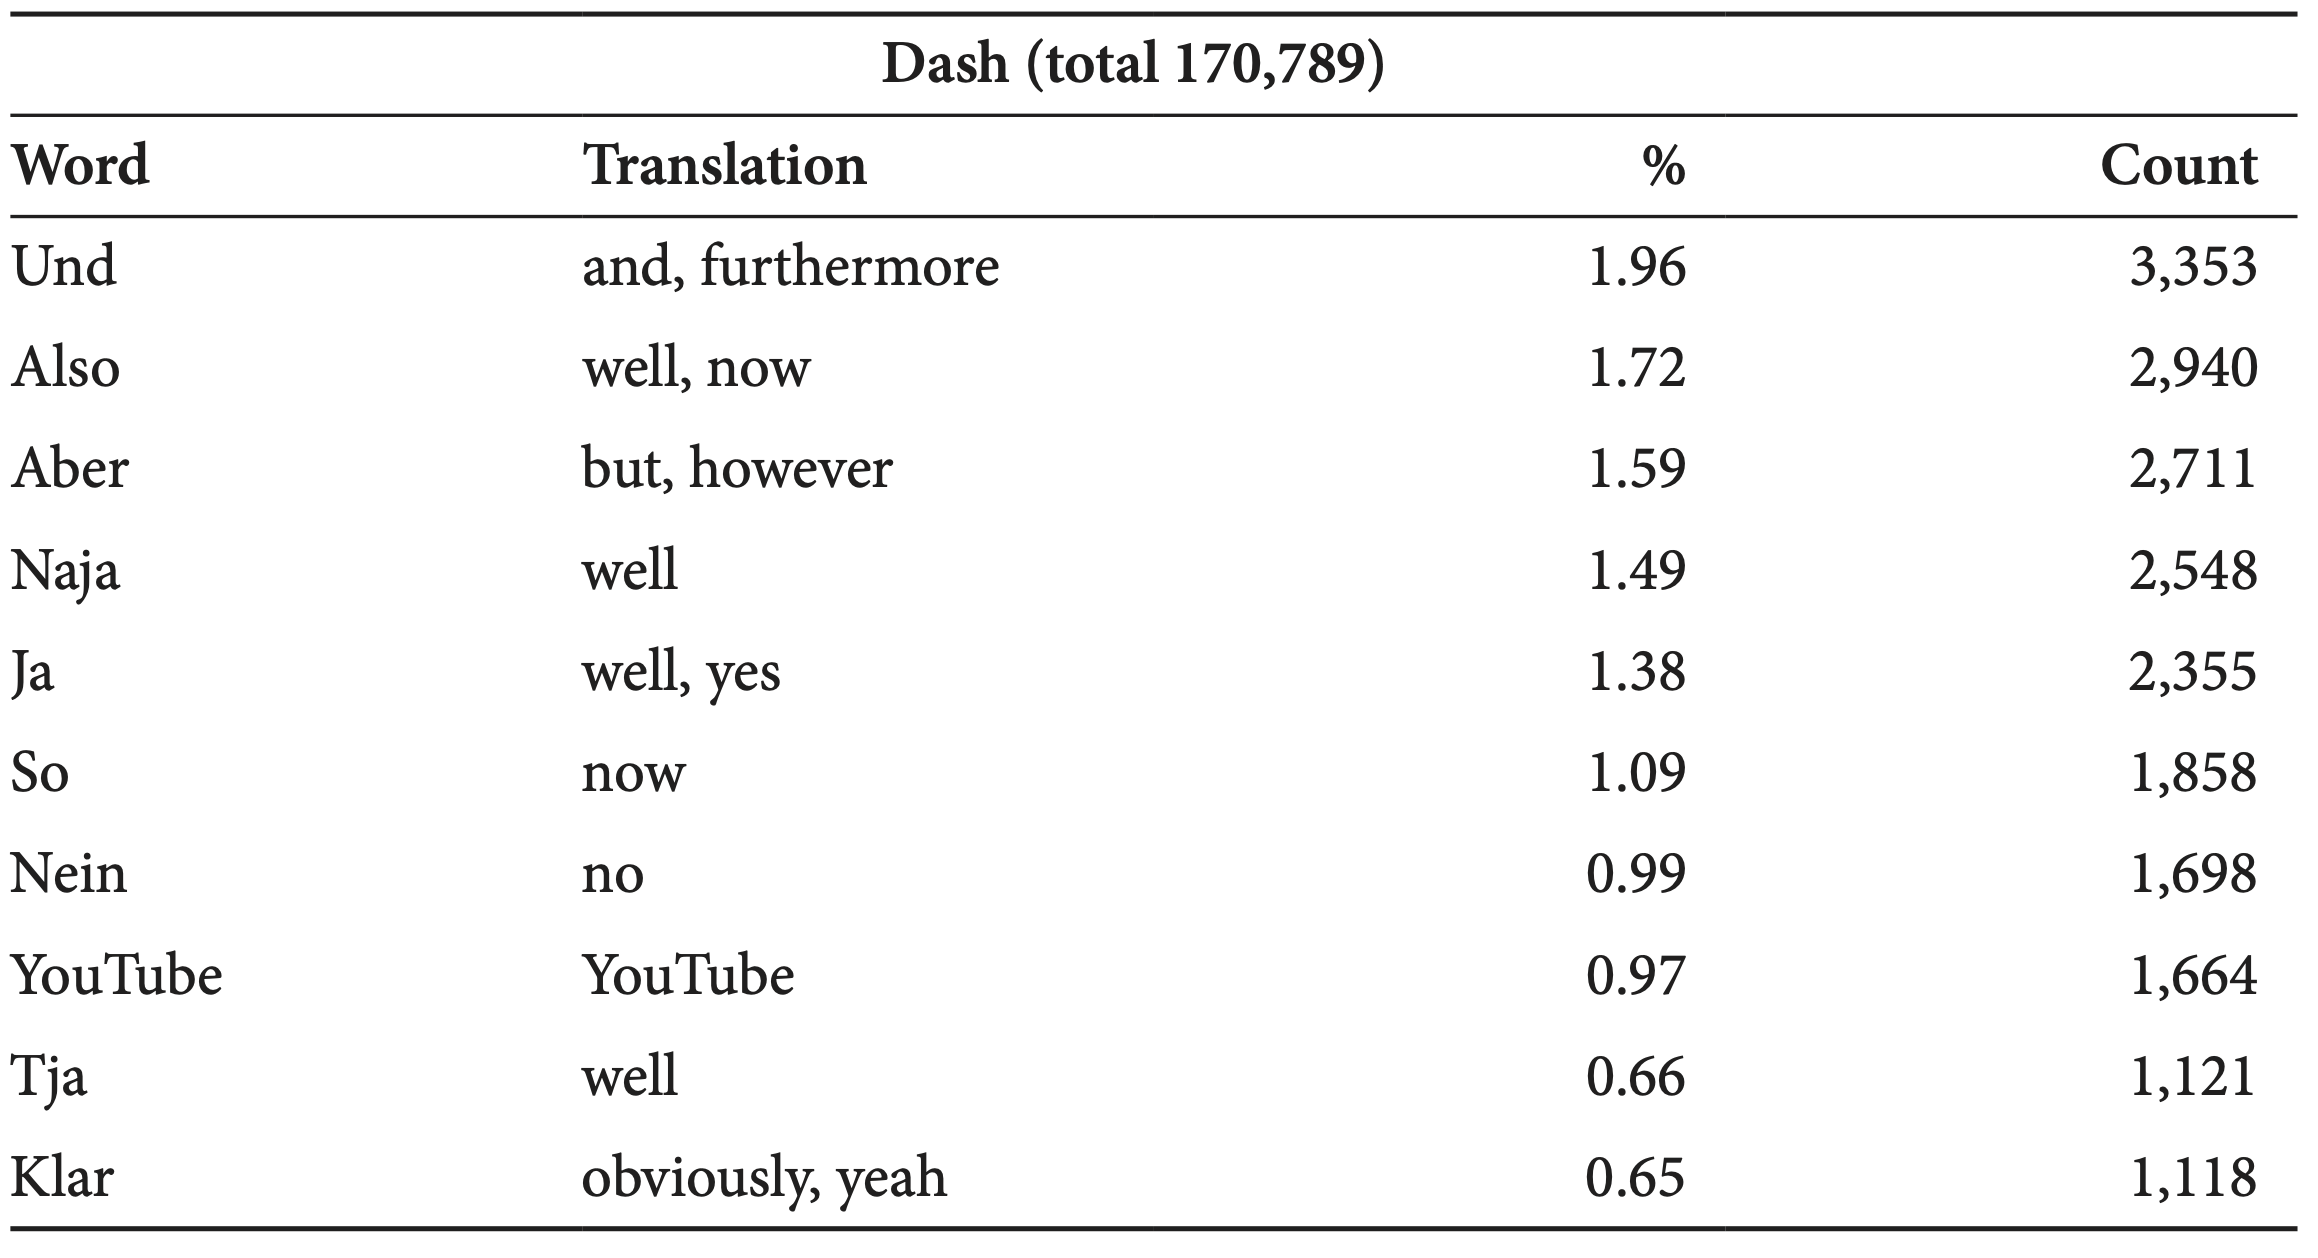
\includegraphics[width=0.7\textwidth]{\GRAPHPATH/obweil/05-dash}
\end{frame}

\begin{frame}
  {Empirischer Befund II/4 | Wortverteilung bei Dreipunkt}
  \centering 
  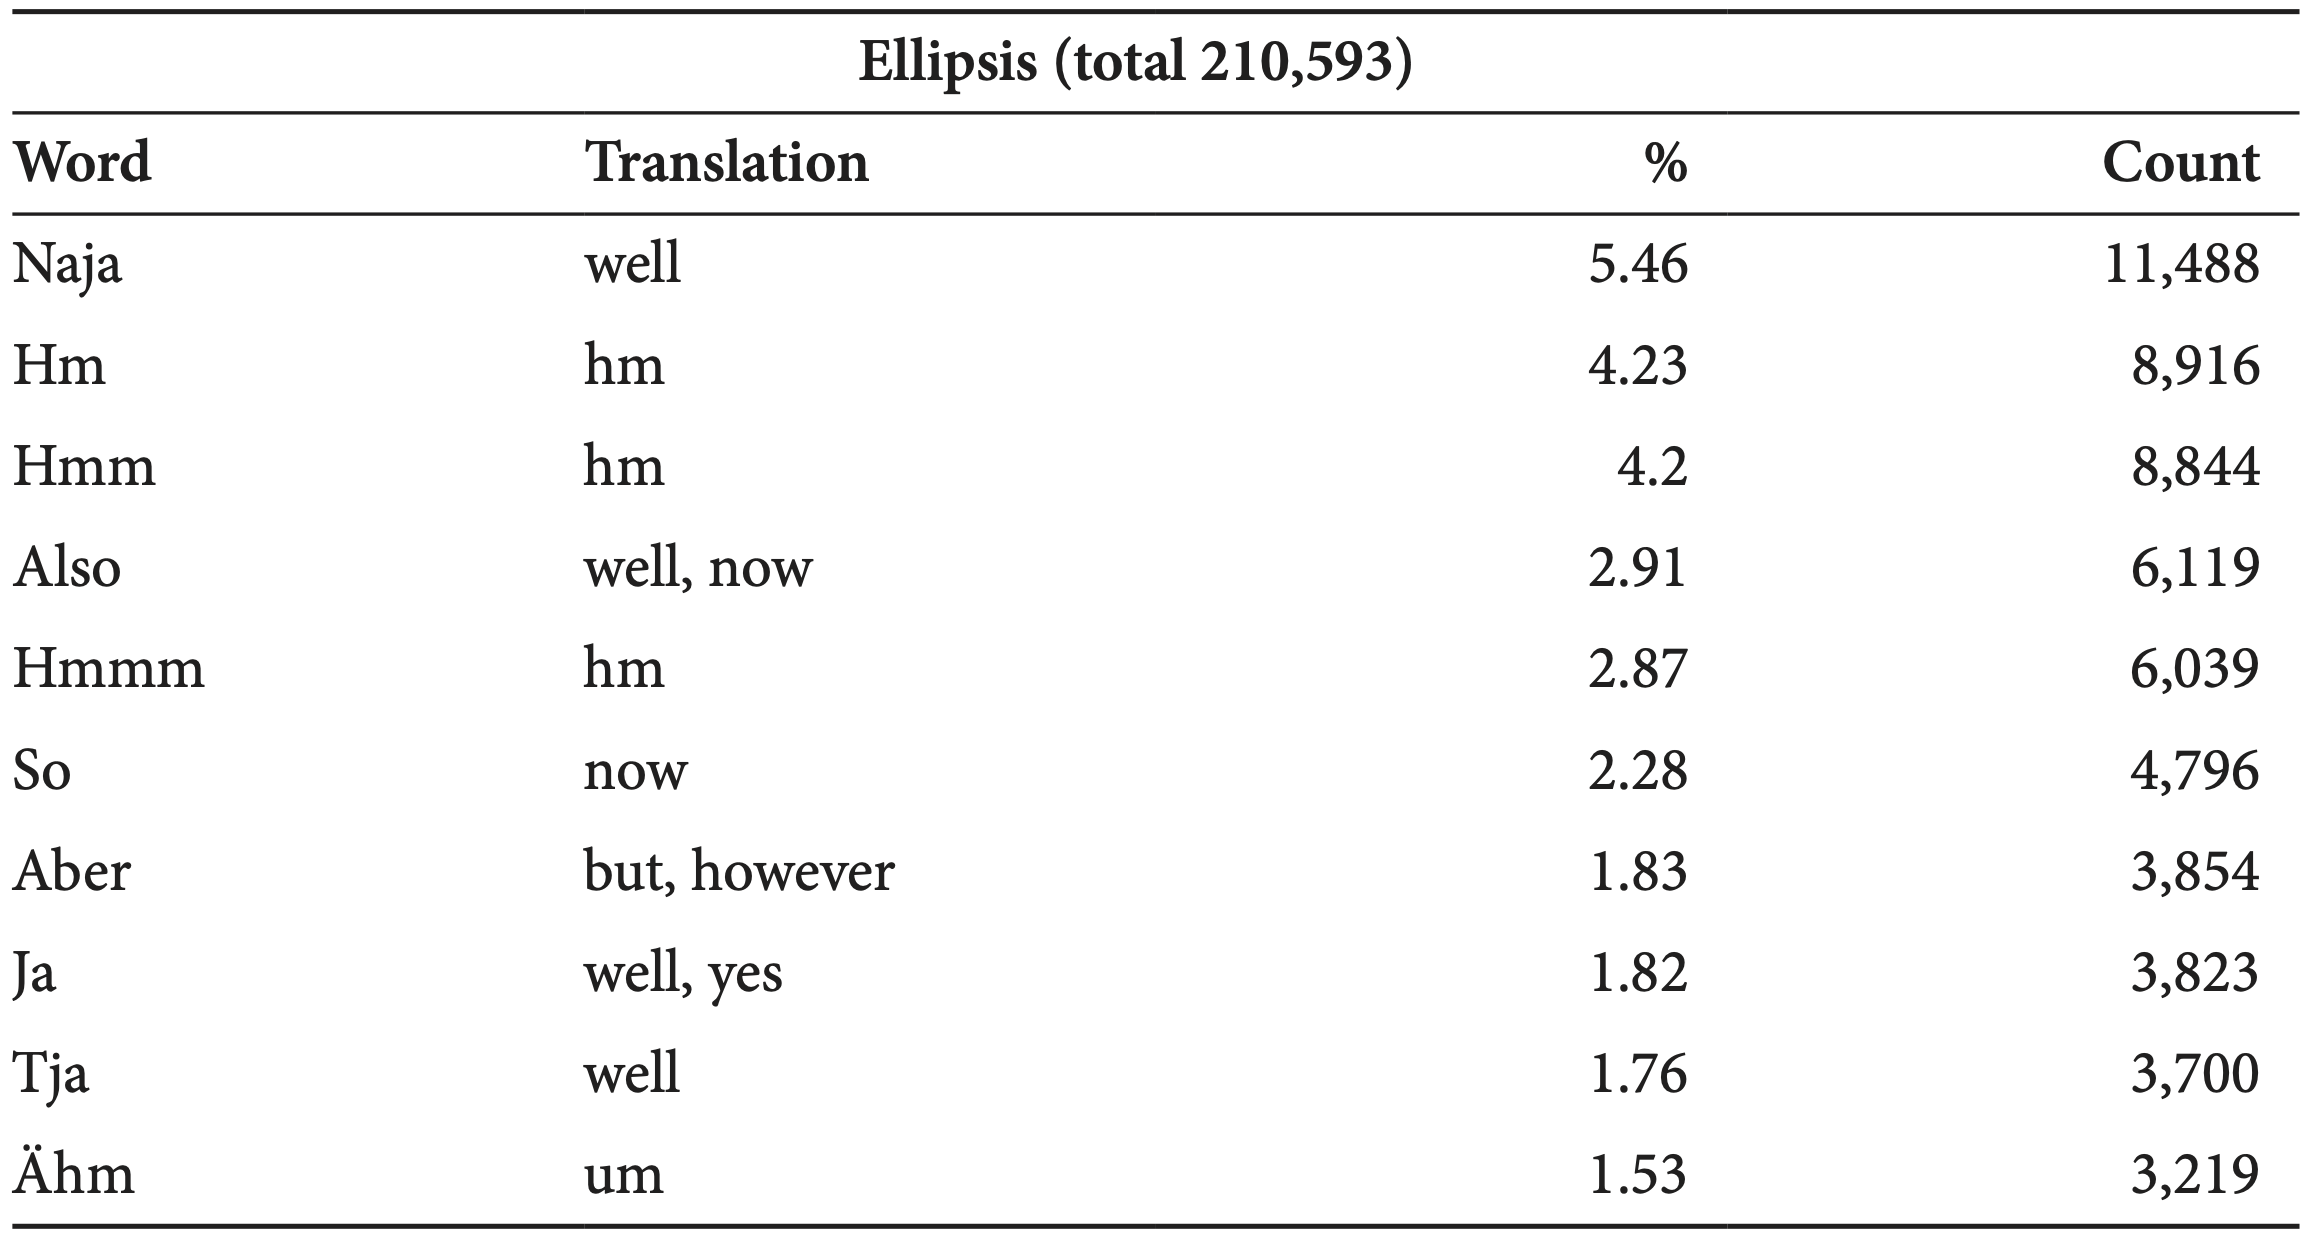
\includegraphics[width=0.7\textwidth]{\GRAPHPATH/obweil/05-ellipsis}
\end{frame}

\begin{frame}
  {Empirischer Befund III/1 | Links von \textit{obwohl}\slash \textit{weil}}
  \centering 
  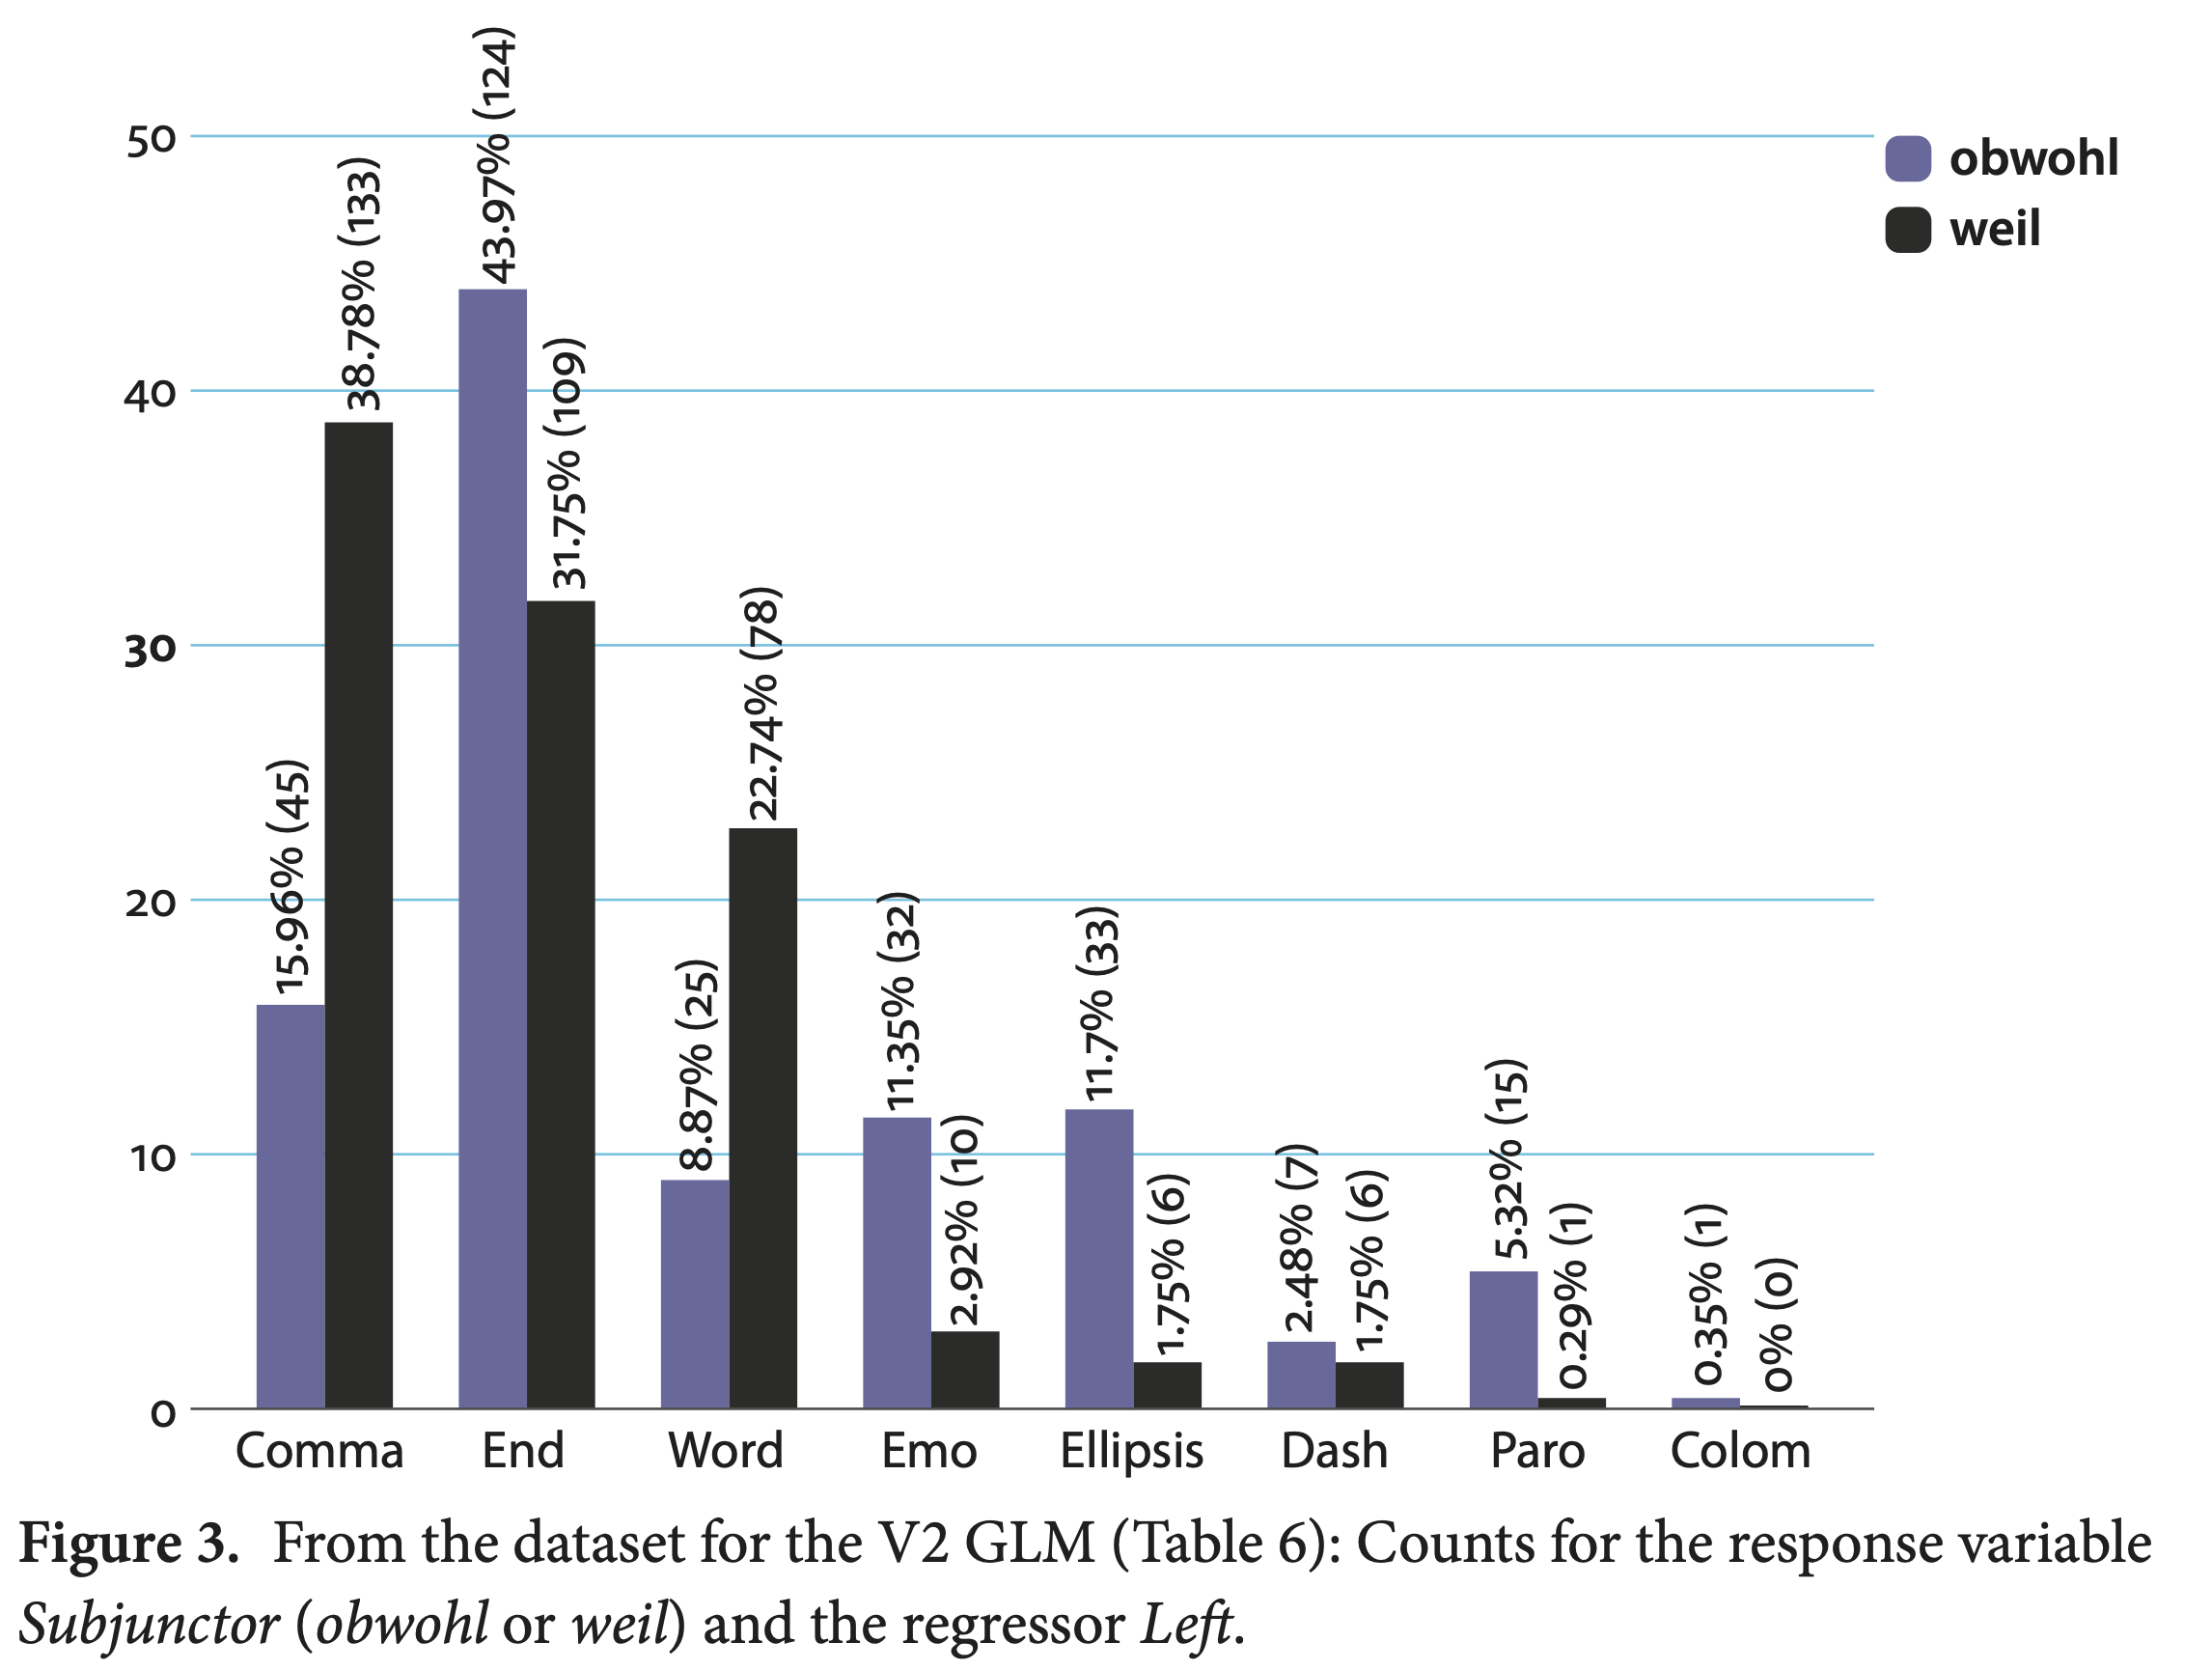
\includegraphics[width=0.7\textwidth]{\GRAPHPATH/obweil/06-left}
\end{frame}

\begin{frame}
  {Empirischer Befund III/2 | Rechts von \textit{obwohl}\slash \textit{weil}}
  \centering 
  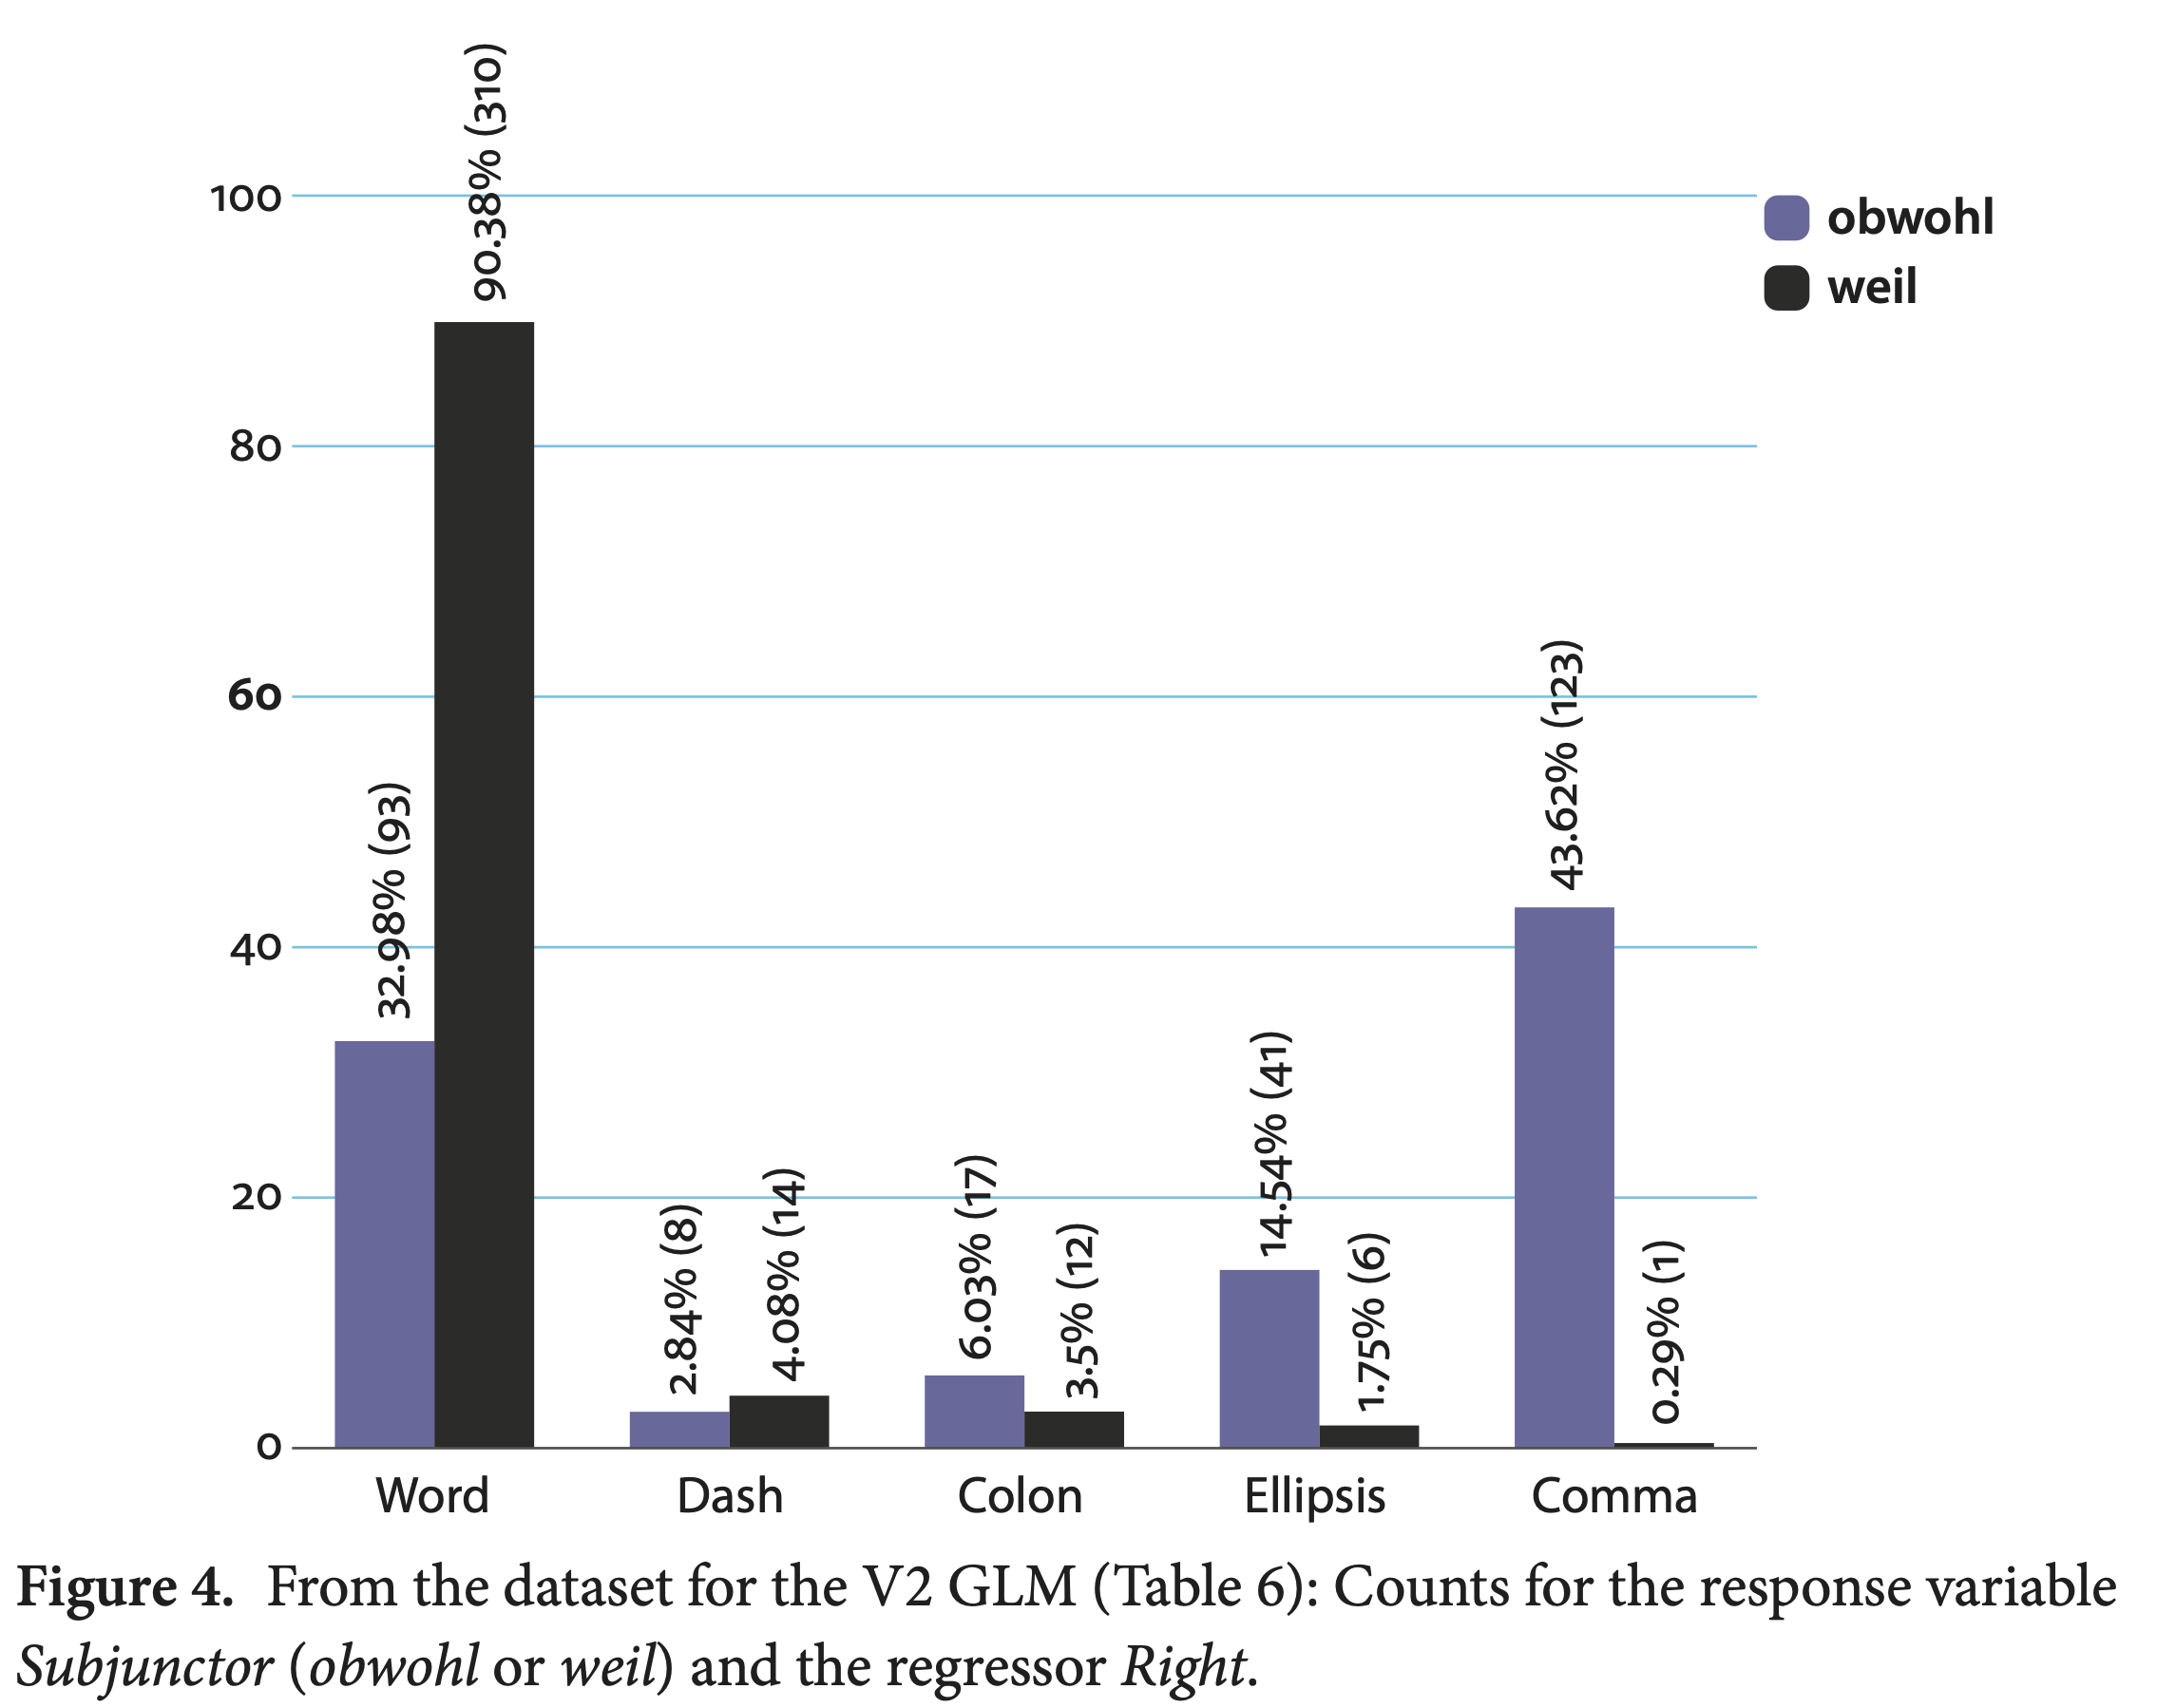
\includegraphics[width=0.7\textwidth]{\GRAPHPATH/obweil/06-right}
\end{frame}

\begin{frame}
  {Ergebnisse}
  \textit{obwohl} und \textit{weil} mit V2-Satzstellung\\
  \Zeile
  \begin{itemize}[<+->]
    \item \textit{obwohl}
      \begin{itemize}[<+->]
        \item leitet mehr unabhängige Sätze ein
        \item wird öfter vom Komma gefolgt
        \item Status | \alert{eher Diskurspartikel außerhalb des Satzes}
        \item ähnlich \textit{ja}, \textit{naja}, \textit{also}, \textit{klar}
      \end{itemize}
      \Zeile
    \item \textit{weil}
      \begin{itemize}[<+->]
        \item folgt auch bei V2 eher einem Komma
        \item oder ganz ohne Interpunktion links
        \item Komma folgt seltener
        \item Status | \alert{eher Konnektor im Konnektorfeld}
        \item ähnlich \textit{denn}
      \end{itemize}
  \end{itemize}
\end{frame}
